\documentclass{lehramt-informatik-haupt}
\liLadePakete{syntax}
\usepackage{tikz}
\usetikzlibrary{shapes.multipart,positioning,fit}

\begin{document}

%%%%%%%%%%%%%%%%%%%%%%%%%%%%%%%%%%%%%%%%%%%%%%%%%%%%%%%%%%%%%%%%%%%%%%%%
% Theorie-Teil
%%%%%%%%%%%%%%%%%%%%%%%%%%%%%%%%%%%%%%%%%%%%%%%%%%%%%%%%%%%%%%%%%%%%%%%%

\chapter{InsertionSort: Sortieren durch Einfügen}

\begin{liQuellen}
\item \cite[Seite 41]{aud:fs:tafeluebung-11}
\item \cite{wiki:insertionsort}
\item \cite[Seite 125-127 (PDF 143-145)]{saake}
\end{liQuellen}

Bei dem InsertionSort-Verfahren muss ein Element gemerkt werden. Dadurch
wird eine Position in der Folge frei, die genutzt werden kann, um alle
Elemente, die größer als das gemerkte Element sind, eine Position nach
rechts zu verschieben. Das Verschieben erfolgt ausgehend von der
aktuellen Position $j$ rückwärts bis zum ersten Element. Ist das Element
$j - 1$ kleiner oder gleich dem gemerkten Element, wird die innere
Schleife verlassen. Durch das Verschieben „nach rechts“ wird die
Position $j$ in der Folge frei, an der das gemerkte Element eingefügt
werden muss.\footcite[Seite 125]{saake}

\def\pfeil#1#2{\draw[-latex] ([xshift=1mm]a.#1 north) -- ++(0,0.25) -| ([xshift=-1mm]a.#2 north);}

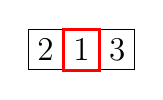
\begin{tikzpicture}[my shape/.style={
  draw,
  font=\large,
  rectangle split horizontal,
  rectangle split parts=3,
  rectangle split,
}]
\node [my shape] (a) {2 \nodepart{two} 1 \nodepart{three} 3};

\node[draw=red, very thick, fit=(a.one split south) (a.two split north), inner sep=0pt] {};

% \node at (a.two split north){n};
% \node at (a.one split south){s};

\pfeil{one}{two}
\pfeil{two}{three}
\end{tikzpicture}

\begin{itemize}
\item Funktionsweise:

\begin{itemize}
\item solange zu sortierende Liste mehr als ein Element beinhaltet:

\begin{itemize}
\item lösche das \emph{erste Element} aus der Liste
\item füge \emph{gemäß Sortierordnung} in die Ergebnisliste ein
\item wiederhole, bis Eingangsliste leer
\end{itemize}

\end{itemize}

\item Eigenschaften von InsertionSort:

\begin{itemize}
\item Laufzeitkomplexität:

\begin{itemize}
\item $\mathcal{O}(n)$ (im Best-Case)
\item $\mathcal{O}(n^2)$ (im Average- und Worst-Case)
\end{itemize}

\item \emph{stabil}
\item bei Arrays \emph{in-situ}
\end{itemize}

\end{itemize}

\liJavaDatei[firstline=9,lastline=34]{sortier/InsertionSort}
\footcite[Seite 125 - 127]{saake}

\section{Zustand des Eingabefelds an einem Beispiel}

\begin{minted}{md}
for: i=1
for (Anfang) 7 4 9 2 3
while        7 7 9 2 3
for (Ende)   4 7 9 2 3
for: i=2
for (Anfang) 4 7 9 2 3
for (Ende)   4 7 9 2 3
for: i=3
for (Anfang) 4 7 9 2 3
while        4 7 9 9 3
while        4 7 7 9 3
while        4 4 7 9 3
for (Ende)   2 4 7 9 3
for: i=4
for (Anfang) 2 4 7 9 3
while        2 4 7 9 9
while        2 4 7 7 9
while        2 4 4 7 9
for (Ende)   2 3 4 7 9
\end{minted}

\liPseudoUeberschrift{Rekursiver Insertionsort}

\liJavaDatei[firstline=36,lastline=60]{sortier/InsertionSort}

\literatur

\end{document}
